\section{Tissue Probability Maps}

% Using the 10 tissue segmentations and their associated MR images, create a groupwise mean template and associated tissue probability maps that are representative of this population. Describe the process and justify your choice of transformation model (rigid, affine and/or non-rigid) [15].


Tissue Probability Maps (TPMs) of cerebrospinal fluid (CSF), gray matter (GM), white matter (WM) and background must be generated so that they can be used as spatial priors for tissue segmentation. For that, the group of subjects with an associated label map representing a previous tissue segmentation has been used.


\subsection{Groupwise registration}
The TPMs are calculated as an average of all the label maps that have been projected to a common space defined by a \textit{template} image. An example of such a template is the one built at the Montreal Neurological Institute (MNI) \cite{evans_3d_1993}. However, for this project a template space has been built iteratively using a groupwise coregistration of all the subjects in the group. All the registrations have been performed using NiftyReg \cite{modat_global_2014}\footnote{The repository containing the Python code used for the experiments and the \LaTeX\ code used to create this report is available online at \href{https://github.com/fepegar/ipmi-coursework}{https://github.com/fepegar/ipmi-coursework}. It was made public at the deadline.}.


\subsubsection{Rigid coregistration}
First, the T1-weighted image of one segmented subject is taken as reference and the rest of the subjects are registered to the reference one by one using rigid registration, i.e. 6 degrees of freedom (DOF) representing translation and rotation. The floating images are resampled to the reference space using sinc interpolation and averaged in order to generate the initial version of the template image. For visualisation purposes, the label maps have also been transformed to the reference space using nearest-neighbor interpolation, and the results have been averaged label by label, yielding an initial version of the TPMs. Figure \ref{fig:template-rigid} shows the results of this initial coregistration step.

\begin{figure}
  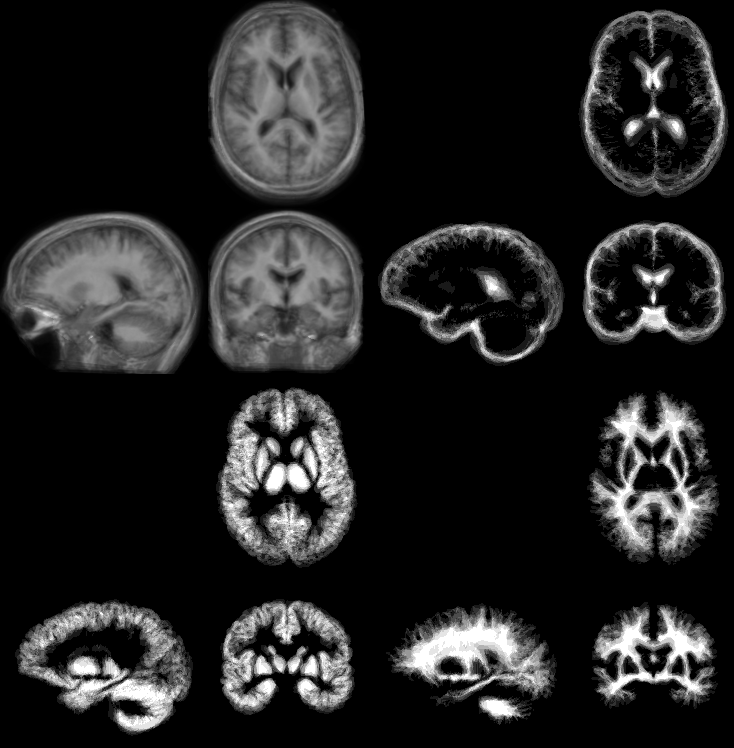
\includegraphics[width=\textwidth]{figures/rigid_template_collage}
  \caption{Results of the rigid coregistration. Top left: mean of the T1-weighted images; top right: TPM of the CSF; bottom left: TPM of the GM; bottom right: TPM of the WM.}
  \label{fig:template-rigid}
\end{figure}

Using only rigid registration for the initial helps reduce the bias of the template. If the first coregistration were performed with using affine registrations (12 DOF representing translation, rotation, shearing and anisotropic scaling), the consecutive iterations would be biased towards the reference image.


\subsubsection{Iterative affine coregistration}
Once a first version of the template is created, it can be used as reference for the following iterations of the coregistration process. This iterative process created a template image and TPMs that were sharper for each iteration, but did not converge to a final result. Up to 10 iterations, the smoothness reduction stopped being visually perceptible. However, the image seem to diverge towards a sheared version of the template after 10 iterations. Figure \ref{fig:template-sheared} shows a comparison between the template image after 10 and 20 iterations and Figure \ref{fig:template-final} shows the final template after 10 affine iterations.


\begin{figure}
  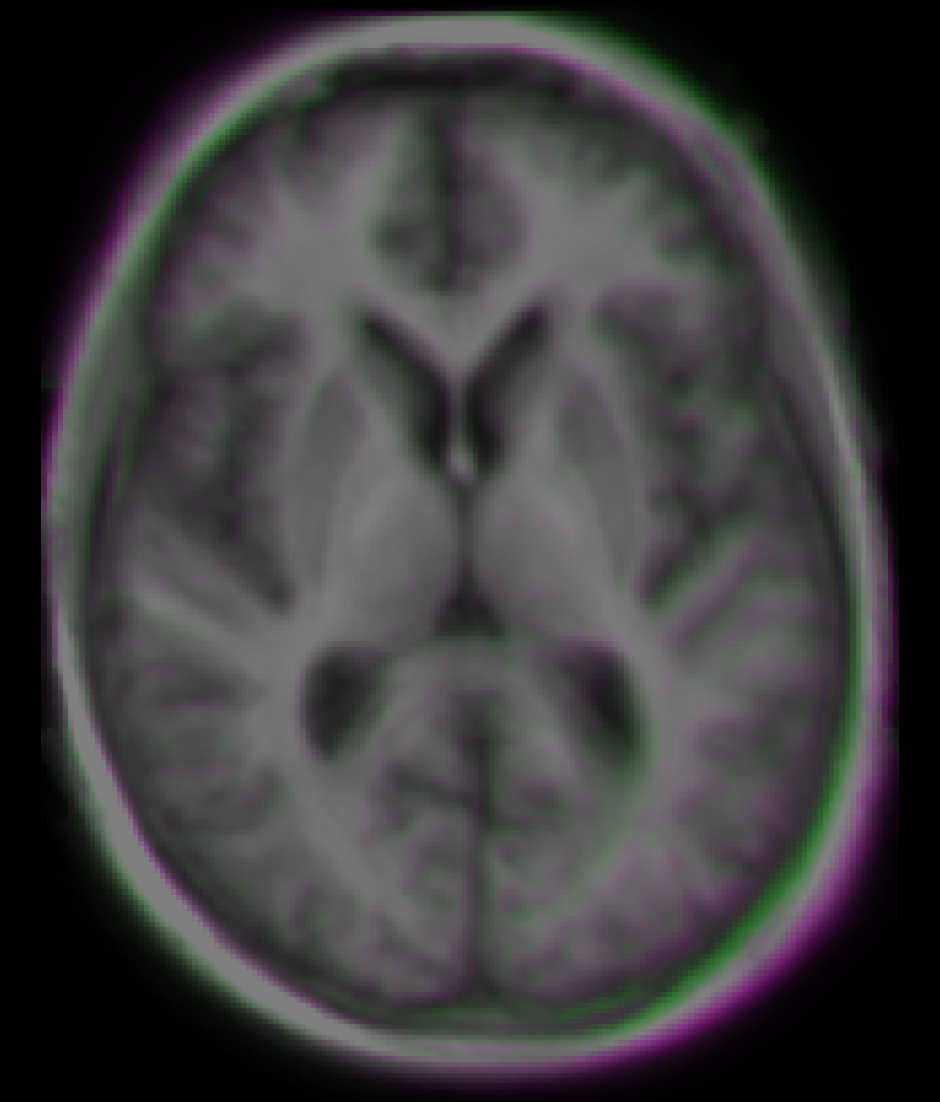
\includegraphics[width=0.5\textwidth]{figures/template_sheared}
  \centering
  \caption{Final template after 10 affine iterations. Top left: mean of the T1-weighted images; top right: TPM of the CSF; bottom left: TPM of the GM; bottom right: TPM of the WM.}
  \label{fig:template-sheared}
\end{figure}


\begin{figure}
  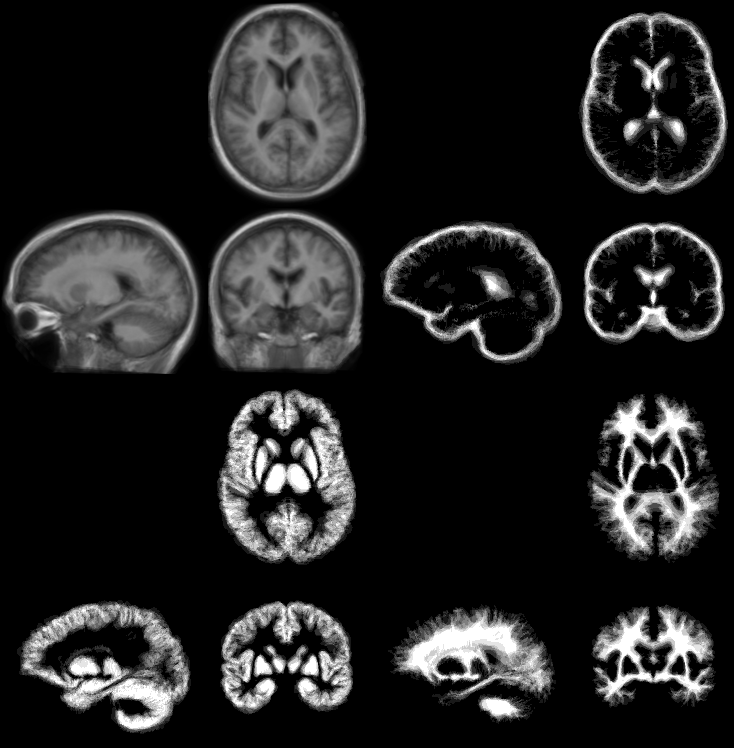
\includegraphics[width=\textwidth]{figures/affine_template_iter_9_collage}
  \centering
  \caption{Template image after 10 affine registration iterations (green) blended with template image after 20 iterations (magenta). The shearing effect is especially visible at the top left and bottom right parts of the image.}
  \label{fig:template-final}
\end{figure}


Moving forward into running coregistration iterations using a free-form registration would result into sharper TPMs, but this might lead to a poorer tissue segmentation, since the priors might not be general enough. For example, if the probability of one voxel being grey matter is close to 0 in the priors that have been propagated to a subject space, that voxel will be missclassified if it actually corresponds to this tissue in that subject image. Early-stopping at affine registration only makes the tissue smoother, capturing a better adaptability of the model to individual cases. Figure \ref{fig:template-std} shows the standard deviation of the final template across the 10 subjects registered to it. The higher variability in the grey matter means that TPMs should be some enough to generalise properly.

\begin{figure}
  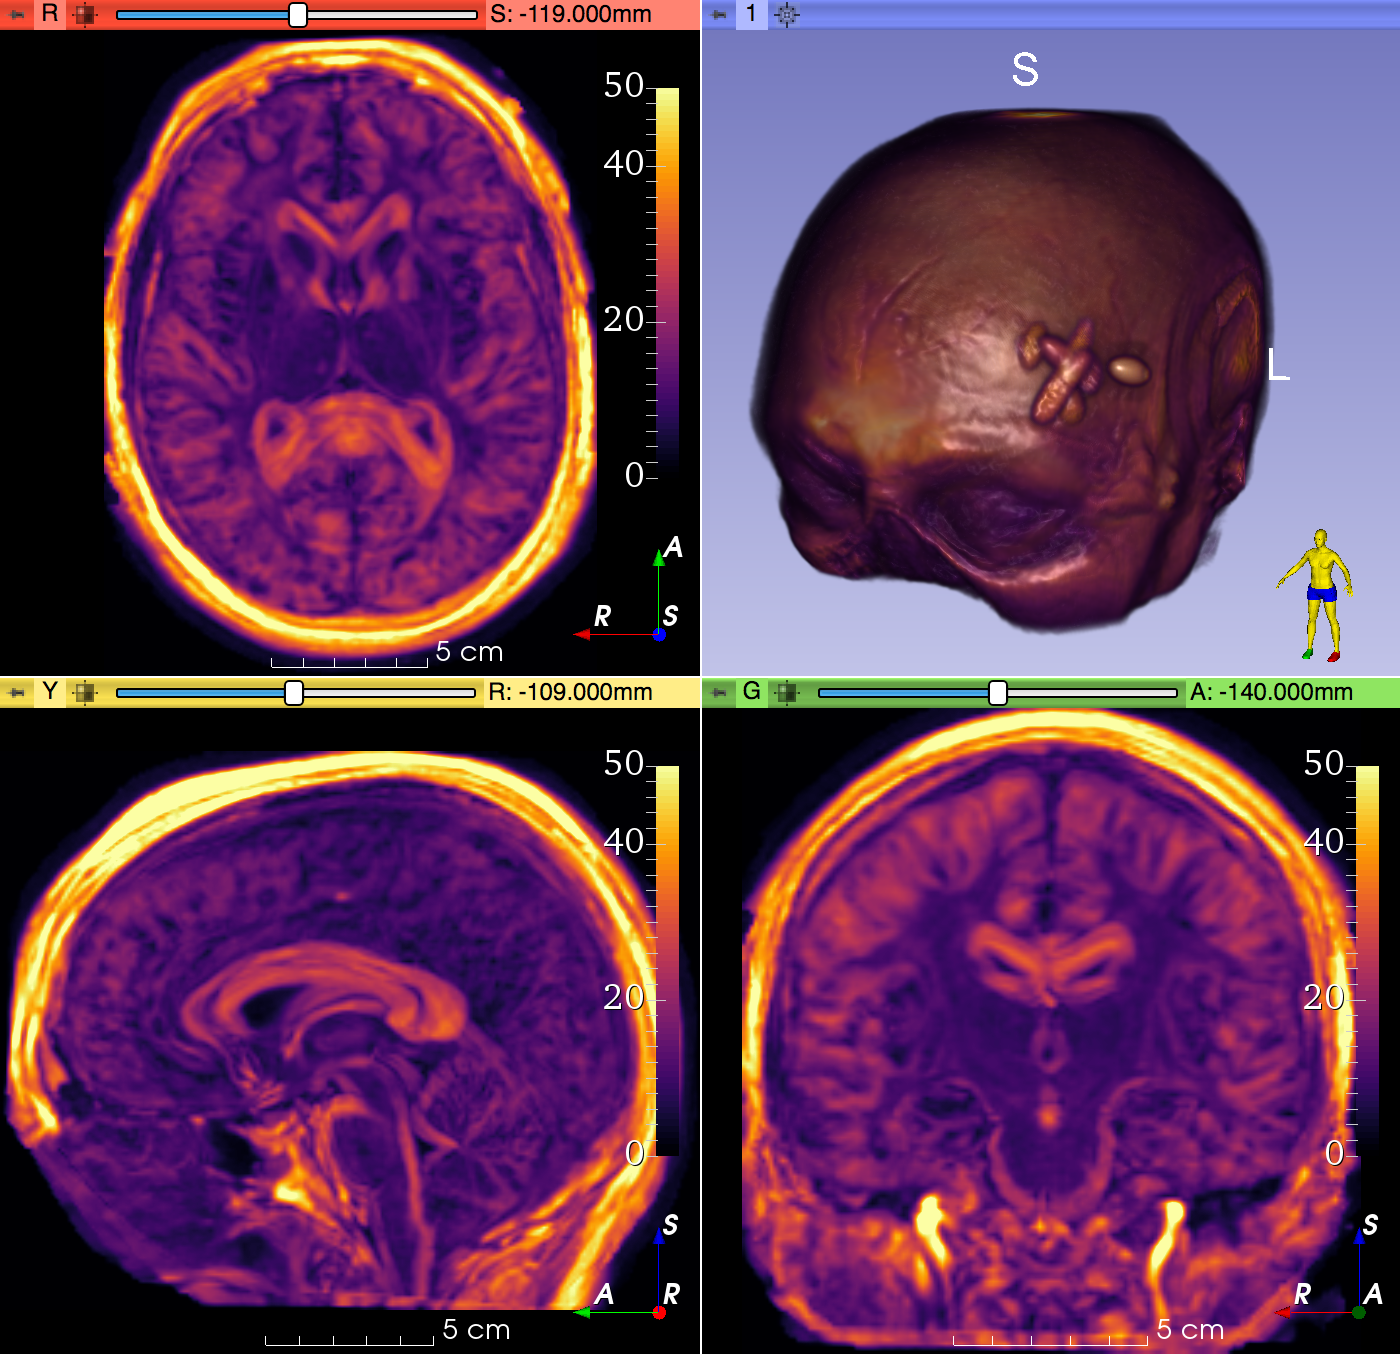
\includegraphics[width=\textwidth]{figures/affine_9_std}
  \centering
  \caption{Standard deviation across the 10 segmented subjects registered to the final template.}
  \label{fig:template-std}
\end{figure}
